\chapter{character assassination}
\label{sec:listing}
\lstset{style=68KStyle}

Writing some text to the screen, such as the copyright information on the title screen, is surprisingly convoluted in its detail,
it will even introduce us to the machinations of the Jaguar's GPU. But although there is a surprising amount of code required from
the developer to get a string of characters onto the display the general principle is one familiar from other platforms: you define
a font, you specify the text you want to display and where you want to display it, and finally you call a routine that will take care of all the detail.

In our case the routine that takes care of all the detail will be our first taste of the implementation and use of what are known as 'shaders', free-standing
programs that are written in a customized version of Motorola 68000 assembly lanage for the Atari's Graphics Procesing Unit(GPU), capriciously dubbed 'Tom' by
the hardware designers of Atari at the time.

Before we get to that we can coast through the relatively easy part of defining our font and specifying our string of text, as well as plugging in the values
to the GPU's buffer that will be required by the shader when it takes care of actually putting pixels on screen.

When it comes to defining a font for the copyright information on Tempest 2000's title screen you may have already guessed where information is contained: in
one of our \icode{beasty} cry files, in this case \icode{beasty4.cry}:

\begin{figure}[H]
    \centering
    \begin{adjustbox}{width=8cm,center}
      \frame{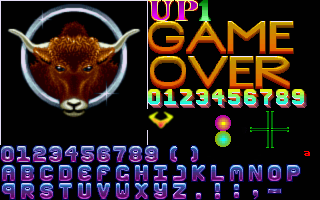
\includegraphics[width=12cm]{src/cry/beasty4.png}}%
    \end{adjustbox}
\caption{\icode{beasty4.cry} with the copyright font at the bottom.}
\end{figure}

And as you may remember the data in \icode{beasty4.cry} is pointed by the variable \icode{pic2}:

\begin{lstlisting}[escapechar=\%]
  pic          EQU $820000          ; beasty3.cry
  pic2         EQU pic+$1f400       ; beasty4.cry
  pic3         EQU pic2+$1f400      ; beasty5.cry
  pic4         EQU pic3+$25800      ; beasty6.cry
  pic5         EQU pic4+(640*128)   ; beasty7.cry
  pic6         EQU pic5+(640*200)   ; beasty8.cry
\end{lstlisting}

So all we have to do to is devise a scheme that maps from a given letter 
or number to its location (and dimensions) in \icode{beasty.cry}.
For example, if we want to display the letter 'A' we need to come up with a way of extracting this:
\begin{figure}[H]
    \centering
    \begin{adjustbox}{width=1cm,center}
      \frame{
\includegraphics[width=1cm]{src/characters/a.png}}%
    \end{adjustbox}
\caption*{A.}
\end{figure}

It helps us that all of our font characters in the \icode{cry} file are the same dimensions so we can make the height and
width a consistent assumption for every glyph. Armed with the location of the pixel data and this dimension information
all that remains is to create a look-up table that tells us the X and Y co-ordinates in \icode{beasty4.cry} for each
character.

The easiest form of look-up table we can make is an 'indexed' one. In other words, a procedure that converts each letter and digit in our character set
into a number that we then use as an index into a list of the X and Y locations. For example, if 'A' is converted to the number 41 then we fetch its
coordinates in \icode{beasty4.cry} from the 42nd member of the list. If 'B' is coverted to number 42 we fetch its co-ordinates from the 43rd member
of the list, and so on. Fortunately we don't have to invent a method of our own for relating letters and digits to a number. The ASCII committee has
done this for us already. So as long as we store the co-ordinates in our list in the same order as given by the ASCII committe we will simply be able
to use the corresponding ASCII value for each letter and digit as our index.

With the main planks of our cunning plan settled in place we can iron out a few details. The best way of storing our co-ordinate information
in this list is to cram the X and Y values into a single place. More specifically, we can assume our X and Y values will always be between
0 and 65,536 so each will fit in one half of a single 4 byte (64 bit value). Another way of describing a value of this length is as a 'long'
and in 68K assembler the notation to denote such a value is \icode{dc.l}.

So let's assume we have 'A' at Y co-ordinate 165 and X co-ordinate 2 in our \icode{beasty4.cry} 'sprite sheet'. Since we're dealing with zero-based indices
we subtract 1 from each of these values to give us 164 and 1 respectively. In hex 164 is \icode{\$A4} and 1 is 
\icode{\$01}. We can fit this into our 4 byte entry as follows:

\begin{figure}[H]
  {
    \setlength{\tabcolsep}{3.0pt}
    \setlength\cmidrulewidth{\lightrulewidth} % Make cmidrule = 
    \begin{adjustbox}{width=3cm,center}
      \begin{tikzpicture}
      \def\BACKGROUNDONE{lightgreen}
      \def\BACKGROUNDTWO{lightblue}
      \fill[\BACKGROUNDONE] (0,0) rectangle ++ (1,1);
      \fill[\BACKGROUNDONE] (1,0) rectangle ++ (1,1);
      \fill[\BACKGROUNDTWO] (2,0) rectangle ++ (1,1);
      \fill[\BACKGROUNDTWO] (3,0) rectangle ++ (1,1);
        \draw[step=1.0,gray,thin] (0,0) grid (1,1);
        \node[matrix of math nodes,anchor=south west,inner sep=0pt,
        nodes={draw,minimum size=1cm,anchor=center},
        column sep=-\pgflinewidth,row sep=-\pgflinewidth,font=\huge\ttfamily]
        {
          00 & A4  & 00 & 01 \\
        };
      \end{tikzpicture}
    \end{adjustbox}
  }
\end{figure}
\vspace{-1cm}

Likewise with our fixed set of dimensions for each of the characters or glyphs. We get out our ruler, apply it to the screen, and determine they
each have a height of 19 and a width of 16. We subtract 1 from each to give us 18 and 15. Convert to hex: \icode{\$12} and \icode{\$0F}. Then
plug them into our 4 byte value:

\begin{figure}[H]
  {
    \setlength{\tabcolsep}{3.0pt}
    \setlength\cmidrulewidth{\lightrulewidth} % Make cmidrule = 
    \begin{adjustbox}{width=3cm,center}
      \begin{tikzpicture}
      \def\BACKGROUNDONE{lightgreen}
      \def\BACKGROUNDTWO{lightblue}
      \fill[\BACKGROUNDONE] (0,0) rectangle ++ (1,1);
      \fill[\BACKGROUNDONE] (1,0) rectangle ++ (1,1);
      \fill[\BACKGROUNDTWO] (2,0) rectangle ++ (1,1);
      \fill[\BACKGROUNDTWO] (3,0) rectangle ++ (1,1);
        \draw[step=1.0,gray,thin] (0,0) grid (1,1);
        \node[matrix of math nodes,anchor=south west,inner sep=0pt,
        nodes={draw,minimum size=1cm,anchor=center},
        column sep=-\pgflinewidth,row sep=-\pgflinewidth,font=\huge\ttfamily]
        {
          00 & 12  & 00 & 0F \\
        };
      \end{tikzpicture}
    \end{adjustbox}
  }
\end{figure}
\vspace{-1cm}
With this information we can now isolate our 'A' glyph and extract it.

\begin{figure}[H]
    \centering
    \begin{adjustbox}{width=7.5cm,center}
      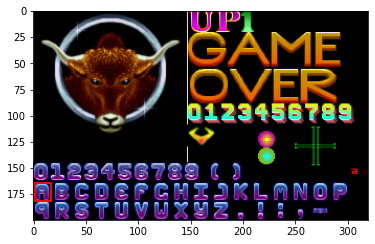
\includegraphics[width=12cm]{src/characters/plot.png}%
    \end{adjustbox}
\caption{The 'A' glyph located in a red box by our dimension and co-ordinate information.}
\end{figure}

The mechanics of our look-up table are now fully worked out so we are ready to create it. Since it has over a hundred entries we store it in 
a separate file called \icode{afont.s} and give it the very descriptive name \icode{afont}. I think this is intended as an abbreviation of
'Atari Font', since it is the font used to write the Atari copyright information. An incomplete excerpt of the file follows below with
ellipses (...) to indicate lines that have been omitted.

\begin{lstlisting}[caption=The opening block of the \icode{afont} data structure in source file \icode{afont.s}.]
*
*
* Page 2 font, by Joby

afont:  
  dc.l pic2      ; pixel data
  dc.l $0012000f ; height ($0012) and width ($000f)

  dc.l $b6011e   ;Space
  dc.l $b600d2   ;!
  dc.l $a40001   ;"
  dc.l $a40001   ;#
  dc.l $a40001   ;$
  dc.l $a40001   ;%
  dc.l $a40001   ;&
  dc.l $a40001   ;'
  dc.l $9100a5   ;(
  dc.l $9100ba   ;)
  dc.l $a40001   ;*
  dc.l $a40001   ;+
  dc.l $b600f8   ;,
  dc.l $b6010b   ;-
  dc.l $b600c2   ;.
  dc.l $a40001   ;/
  ...
  dc.l $a40001  ;A <-- This is the one! Y: $00a4, X: $0001
  dc.l $a40014  ;B
  dc.l $a40027  ;C
  ...
\end{lstlisting}

Notice that the order in which we have defined the location of each character corresponds to the order (or value) of each character
according to the ASCII specification. This means that when we define the text we want to display all we have to do is convert each
character in the text to its corresponding ASCII value '\icode{n}' and get that \icode{n}th value from our \icode{afont} list.

So let's define the text we want to display:

\begin{lstlisting}
ataricop1: dc.b "COPYRIGHT 1981,",0
ataricop2: dc.b "1994 ATARI CORP.",0
\end{lstlisting}

This is straightforward enough. Note that we have a zero at the end of each string. This makes them 'null-terminated' - a feature
that will come in handy later when we need to identify that the end of the string when writing it to the screen.

Now that we have our text defined we can start the process of writing it to the screen. These two concise little paragraphs
do this job for us. Given the amount of info encoded in our \icode{afont} data structure we only need to set up one additional
piece of info for the \icode{centext} routine that will do our heavy lifting. This is the Y position that we want to write
the text to on the screen (adjusted for whether we're on a PAL or NTSC screen).

\begin{lstlisting}
  lea afont,a1      ; Load the font data structure
  lea ataricop1,a0  ; Load the first line of the copyright info
  move #190-8,d0    ; Set the Y position for the text
  add palfix2,d0    ; Adjust for PAL screens 
  jsr centext       ; Write the text                 

  lea afont,a1      ; Load the font data structure
  lea ataricop2,a0  ; Load the second line of the copyright info
  move #207-5,d0    ; Set the Y position for the text
  add palfix2,d0    ; Adjust for PAL screens 
  jsr centext       ; Write the text                 
\end{lstlisting}

The \icode{centext} routine (short for 'center the text')  we call into at the end of each paragraph above is where things start to get detailed. It is still
not the tangled core of this particular beast but it is certainly a busier proposition that anything we've looked at so far.
But we can settle our nerves for the moment because it is in fact doing something quite straightforward:
it is setting up a buffer of data for the GPU to use. It stores this buffer at an address in the GPU RAM given by the \icode{inbuf} variable. This buffer
is a 36 byte array containing the 4-byte addresses of all the different bits of data the GPU will need to render the text. Here
are all the bits and piece in the order that they appear in \icode{inbuf} once \icode{centext} is finished:

\begin{figure}[H]
  {
    \setlength{\tabcolsep}{3.0pt}
    \setlength\cmidrulewidth{\heavyrulewidth} % Make cmidrule = 
    \begin{adjustbox}{width=10cm,center}

      \begin{tabular}{lll}
        \toprule
        GPU RAM Address & Name & Description\\
        \midrule
        \icode{\$F0003F60}   & \icode{ataricop1} & Address in RAM of the text to write\\
        \icode{\$F0003F64}   & \icode{afont} & Address in RAM of the font data structure\\
        \icode{\$F0003F68}   & \icode{\$00000000} & Drop Shadow Vector X axis\\
        \icode{\$F0003F6C}   & \icode{\$00000000} & Drop Shadow Vector Y axis\\
        \icode{\$F0003F70}   & \icode{\$00010000} & Text Scale X axis\\
        \icode{\$F0003F74}   & \icode{\$00010000} & Text Scale Y axis \\
        \icode{\$F0003F78}   & \icode{\$00000000} & Text Shear X axis\\
        \icode{\$F0003F7C}   & \icode{\$00000000} & Text Shear Y axis\\
        \icode{\$F0003F84}   & \icode{\$00B600A7} & Y \& X Co-ordinates to Write Text To\\
        \icode{\$F0003F80}   & \icode{\$00000000} & Drop Shadow Mode Enabled\\
        \bottomrule
      \end{tabular}
    \end{adjustbox}
  }\caption*{The 10 4-byte addresses stored beginning in \icode{inbuf} by \icode{centext}.}
\end{figure}

In addition to the items of data we've collected so far we can see that we plug in a few extras in the \icode{centext}
routine. These are graphical effects such as the scaling to apply to each character, the dimensions of a drop shadow
to apply on each, and finally the 'shear' to apply. 'Shear' distorts an object along the depth or 'Z' axis to make it
appear like we are looking at it at an angle in 3 dimensions. The only one of these parameters we using is the scaling,
for the rest we just plug in zero. But here's what the copyright text would look like with some shear applied:

\begin{figure}[H]
    \centering
    \begin{adjustbox}{width=9cm,center}
      
\includegraphics[width=12cm]{src/characters/shear.png}%
    \end{adjustbox}
\caption{What the characters look like when we apply a shear value of 800 on both the X and Y axes.}
\end{figure}

And here's what they looks like if we bump up the scale on the X and Y axis:

\begin{figure}[H]
    \centering
    \begin{adjustbox}{width=9cm,center}
      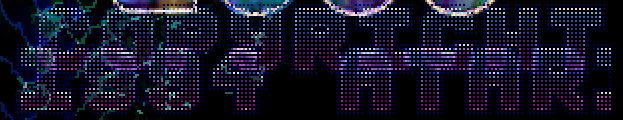
\includegraphics[width=12cm]{src/characters/scale.png}%
    \end{adjustbox}
\caption{What the characters look like when we apply a scale value of 2000 instead of 1000. The pixellated, exploded appearance 
  gives some hint that 'scale' here is not simply concerned with size but a specific 'explosion
  type' effect.}
\end{figure}

We'll encounter effective use of these features elsewhere in Tempest 2000 so won't go any further into them for now.

\begin{lstlisting}[caption=The \icode{centext} routine responsible for setting up the values in our GPU buffer.]
centext:
  move.l a0,d2          ; Store 'text' in d2 so we don't overwrite it.
  lea in_buf,a0         ; Use 'in_buf' as the buffer to write to.
  move.l d2,(a0)        ; Store 'text' in the first position.
  move.l a1,4(a0)       ; Store 'afont' in the 2nd position.
  move.l #0,8(a0)       ; Store 0 in the 3rd position.
  move.l #0,12(a0)      ; Store 0 in the 4th possition (Dropshadow vector).
  move.l #$10000,16(a0) ; Store 10000 in the 5th position (X Text Scale).
  move.l #$10000,20(a0) ; Store 10000 in the 6th position (Y Text Scale).
  move.l #0,24(a0)      ; Store 0 in the 7th position (X Text Shear).
  move.l #0,28(a0)      ; Store 0 in the 8th position (Y Text Shear).
  move.l #0,36(a0)      ; Store 0 in the 10th position.

  ; This paragraph is about figuring out the X pos we want to place
  ; the texta nd then storing that along with the Y pos in the 10th
  ; position in the buffer
  bsr g_textlength ; Get the length of the text in d2 and store it in d7.     
  ; This uses the text length to center it along the X axis and
  ; store the result in d0;
  lsr #1,d7             
  neg d7
  add #192,d7
  ; d0 contains the Y pos, so move it to the left hand side
  ; of the 4 byte word.
  swap d0               
  move d7,d0       ; Move the X pos we've calculated into the right.
  move.l d0,32(a0) ; Move the X/Y pos in the 9th position.

  ; We're now ready to run the GPU.
  lea texter,a0
  jsr gpurun
  jmp gpuwait
\end{lstlisting}

\icode{centext}, given above, stuffs all these items into a buffer of GPU RAM called \icode{in\_buf} and when that is done
loads and runs a separate little GPU module called a 'shader'. In this case the name of the shader program is \icode{texter},
giving us a little clue to its domain of expertise. This shader is a free-standing piece of code written in a slightly different
flavour of 68000 assembly language. Despite it's name \icode{texter} is contained in a source file called \icode{stoat.gas}. (Nearly
all of the shaders, like the main program source file, are named after beasts of one sort or another. There is no logic or convention
that can be applied to the names. They're just a bit of fun.)

\begin{lstlisting}
texter:
	.incbin 	"bin/stoat.o"
\end{lstlisting}

\icode{texter} is slightly more than just a 'writing strings to the screen' routine. In addition to deforming the text as we saw in the
'shear' example above, it can also 'explodes' the text using the 'scale' parameters. A comment near the top of \icode{stoat.gas} (the
source file for the \icode{texter} routine) tells the possible inspiration for this effect:

\begin{lstlisting}
;*****
;*
;* REX: Robotron explosion generator. Takes an image from the source screen and expands
;* it in X and Y, then uses a1_n to draw the resultant matrix of single pixels.
;*
;*  Provide: dest screen in gpu_screen, in_buf: 0=source image address
;*  4=source image start pixel address, 8=x and y size of source, 12=X scale (16:16),
;*  16=Y scale (16:16), 20=X shear (16:16), 24=Y shear,
;*  28=Mode (0=Top edge, 1=Centered), 32=Dest X and Y 
;*
;*****
\end{lstlisting}

The 'robotron explosion' is the effect visible below. As you gradually dial up the X and Y scale parameters and call this shader at each
iteration it can appear as though the text is 'exploding' outwards. There is no real mystery to how the shader writes our characters
to the screen. It uses the same blitting operation we covered previously but with the difference that the preparation of the blitting command
and all the special calculations we might want to do if adding shear, scaling and drop shadows in advance of calling the blitter are done from
within the special purpose processor of the GPU rather than in the CPU. The reason for doing it this way is because the GPU is designed to be fast
at a small number of arithmetic operations such as adding and multiplying so if we're going to do a lot of them and don't want to slow the
rest of the game down, the GPU is the man for our job. We'll next take a look at the internals of the \icode{texter} shader, including the 
relatively trivial task of blitting our characters to the screen, in the next chapter.

\begin{figure}[H]
    \centering
    \begin{adjustbox}{width=9cm,center}
      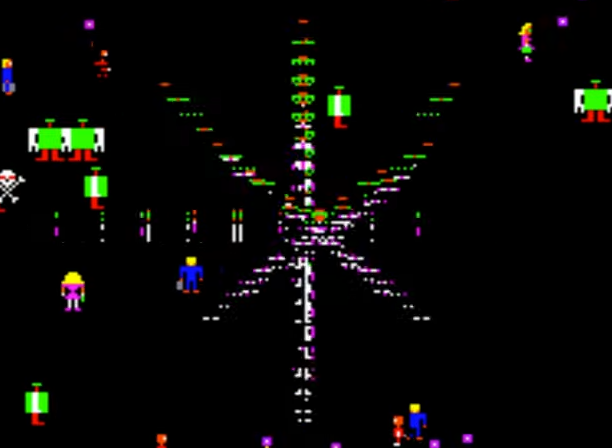
\includegraphics[width=12cm]{src/characters/robotron.png}%
    \end{adjustbox}
\caption{The explosion effect in 'Robotron 2084'.}
\end{figure}


